\documentclass[11pt,class=report,crop=false]{standalone}
\usepackage{exo7hilisit}

\begin{document}


\entete{Hilisit}{Capacité mathématiques}

\titre{\'Equations différentielles -- Partie 2 : Notion d'équation différentielle} 

\bigskip
\bigskip


%%%%%%%%%%%%%%%%%%%%%%%%%%%%%%%%%%%%%%%%%%%%%%%%%%%%%%%%%%%%
%\section{Notion d'équation différentielle}


\exercice{}
\enonce
Vérifier que les fonctions $f$ suivantes sont solutions de l'équation différentielle donnée.
\begin{enumerate}
  \item $f(x) = -e^{2x}$, $y'=2y$.
  \item $f(x) = \frac{1}{2-x}$, $y'=y^2$.
  \item $f(x) = (3+2x)e^x$, $y''-2y'+y=0$.
  \item $f(x) = Ce^{-x}+\sin(x)-\cos(x)$ (quelle que soit la constante $C$), $y'+y=2\sin(x)$
\end{enumerate} 
\finenonce

\finexercice


\exercice{}
\enonce
Déterminer toutes les solutions constantes des équations différentielles suivantes.
\begin{enumerate}
  \item $y'+y=5$
  \item $y'=y^2-y$
  \item $y'=y^2-4y+1$
  \item $y' = y + x$
\end{enumerate} 
\finenonce

\finexercice


\exercice{}
\enonce

Le dessin représente quelques solutions de l'équation différentielle $y'=y-1$.

\begin{center}
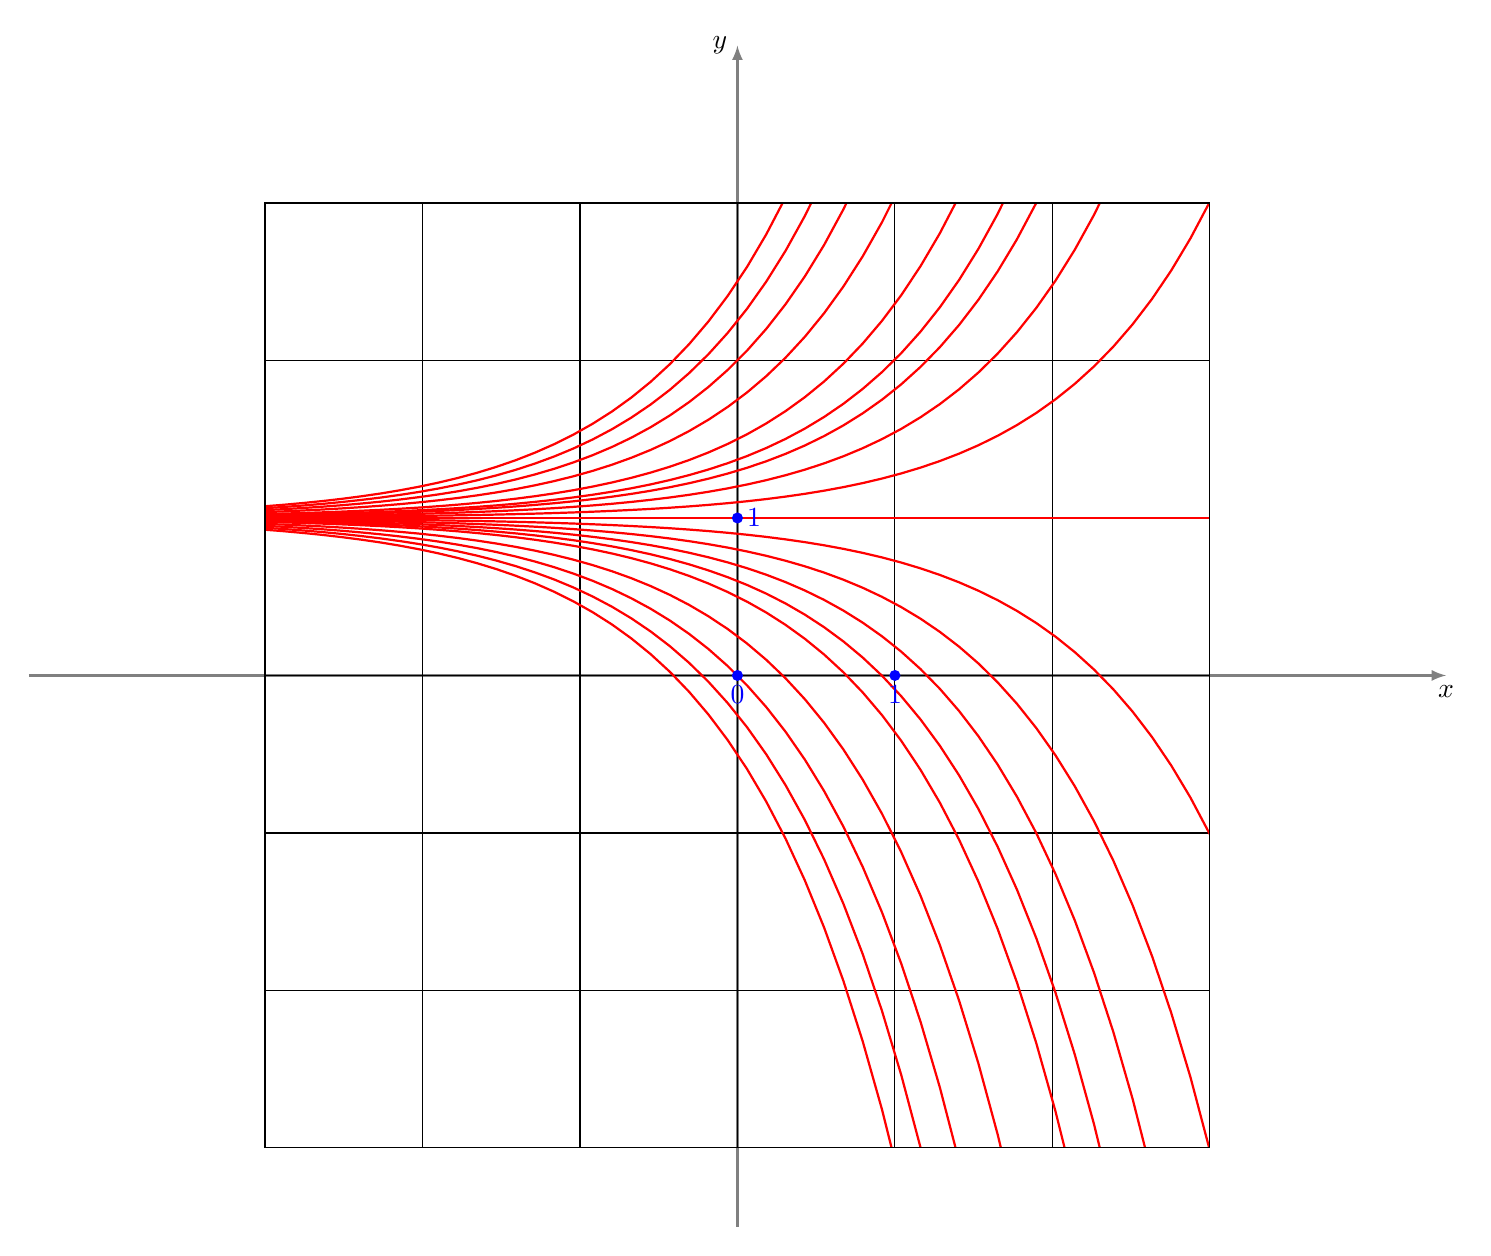
\begin{tikzpicture}[scale=2]

  \draw[->,>=latex,thick,gray] (-4.5,0) -- (4.5,0) node[below,black] {$x$};
  \draw[->,>=latex,thick,gray] (0,-3.5) -- (0,4) node[left,black] {$y$};
  \draw (-3,-3) grid (3,3);
\begin{scope}
    \clip (-3,-3) rectangle (3,3);


\foreach \k in {-1.5, -1.25,-1,-0.75,-0.5,-0.4,-0.3,-0.2,-0.1,0,0.1,0.2,0.3,0.37,0.5,0.75,1,1.25,1.5} {
  \draw[thick, color=red,domain=-3:3, samples=50] plot (\x,{\k*exp(\x)+1});
}

\end{scope}

\fill[blue] (0,0)  circle (1pt) node [below] {$0$}; 
\fill[blue] (1,0)  circle (1pt) node [below] {$1$}; 
\fill[blue] (0,1)  circle (1pt) node [right] {$1$};

\draw (-3,-3) rectangle (3,3);

\end{tikzpicture}
\end{center}


\begin{enumerate}
  \item Répondre graphiquement aux questions suivantes :
  \begin{enumerate}
    \item Quelle est la limite d'une solution en $-\infty$ ?
    \item Quelle est la solution constante ?
    \item En fonction de la valeur $f(0)$ d'une solution $f$, discuter si $f$ est croissante ou décroissante et déterminer la limite en $+\infty$.
    \item Tracer la tangente à la courbe solution qui passe par le point $(0,2)$ ; en déduire une équation approchée de cette tangente.
    \item Tracer la tangente à la courbe solution qui passe par le point $(1,-1)$ ; en déduire une équation approchée de cette tangente.
  \end{enumerate} 


  \item  Répondre par le calcul aux questions suivantes (il n'y a pas besoin de résoudre l'équation) :

  \begin{enumerate}
    \item Soit $f$ la solution dont le graphe passe par le point $(0,0)$. Combien vaut $f(0)$ ? Combien vaut $f'(0)$ ? En déduire la pente de la tangente en ce point, puis l'équation de cette tangente.

    \item  Soit $g$ la solution dont le graphe passe par le point $(1,2)$. Combien vaut $g(1)$ ? Combien vaut $g'(1)$ ? En déduire l'équation de la tangente en ce point.
  \end{enumerate} 

\end{enumerate} 
\finenonce

\finexercice


\exercice{}
\enonce
Une tasse de café de température $T_0= 100$ degrés Celsius
est posée dans une pièce de température $T_\infty = 20$ degrés.
La loi de Newton affirme que la vitesse de décroissance de la température
est proportionnelle à l'écart entre sa température
$T(t)$ et la température ambiante $T_\infty$.

Sachant qu'au bout de $3$ minutes la température du café
est passée à $80$ degrés, quelle sera sa température au bout de $5$ minutes ?

Les questions détaillent les étapes de la résolution de ce problème :

\begin{enumerate}
  \item Justifier que la fonction température $T(t)$ satisfait l'équation différentielle 
$y' = -k(y-20)$ pour une certaine constante $k>0$.

  \item Vérifier que $T(t) = Ce^{-kt}+20$ est solution de cette équation différentielle pour toute constante $C$.

  \item Calculer $C$ en fonction de $T(0)$.

  \item Quelle est la température au bout d'un temps très long ?

  \item Déterminer la constante $k$ en utilisant que $T(3)=80$.

  \item Trouver la solution du problème.
\end{enumerate} 
\finenonce

\finexercice


\end{document}
